\chapter{3D phase tracking Monte Carlo algorithm}

\section{Introduction}

\section{Theory}

In order to simulate Bessel beams, which rely on interference effects, we first must introduce the concept of phase into our \gls{mcrt} simulation. As stated in~\cref{sec:mcrt}, \gls{mcrt} is a technique that simulates particles, thus simulating any wave like behaviour requires additions to the simulations. We achieve this by tracking the phase of photon packets. 

\begin{equation}
I(\xi)=\left| \sum\limits_{\xi}cos\left(\frac{2\pi d}{\lambda}\right) + i \sum\limits_{\xi}sin\left(\frac{2\pi d}{\lambda}\right)\right|^2,\ \ \ \xi=(x,y,z)
\end{equation}

\noindent Where:

\indent $d$ is the total distance travelled by a photon;

\indent $\lambda$ is the wavelength of the photon;

\indent $I$ is the intensity at the $\xi^{th}$ cell.

\medskip

\begin{figure}
\centering
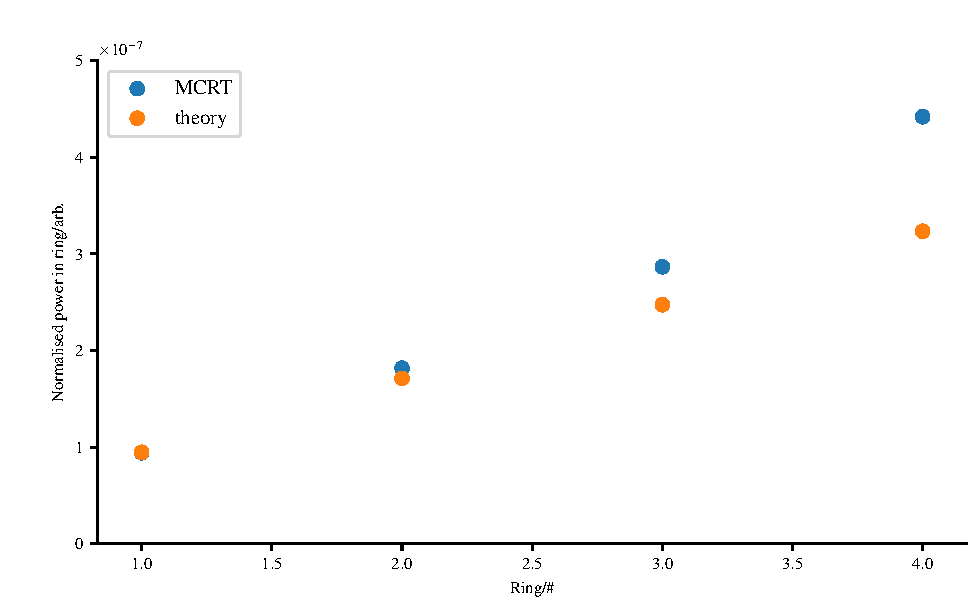
\includegraphics[scale=0.65]{pwr-rings.pdf}
\caption{Bessel beam power in each ring.}
\label{fig:pwrring}
\end{figure}

\begin{figure}
\centering
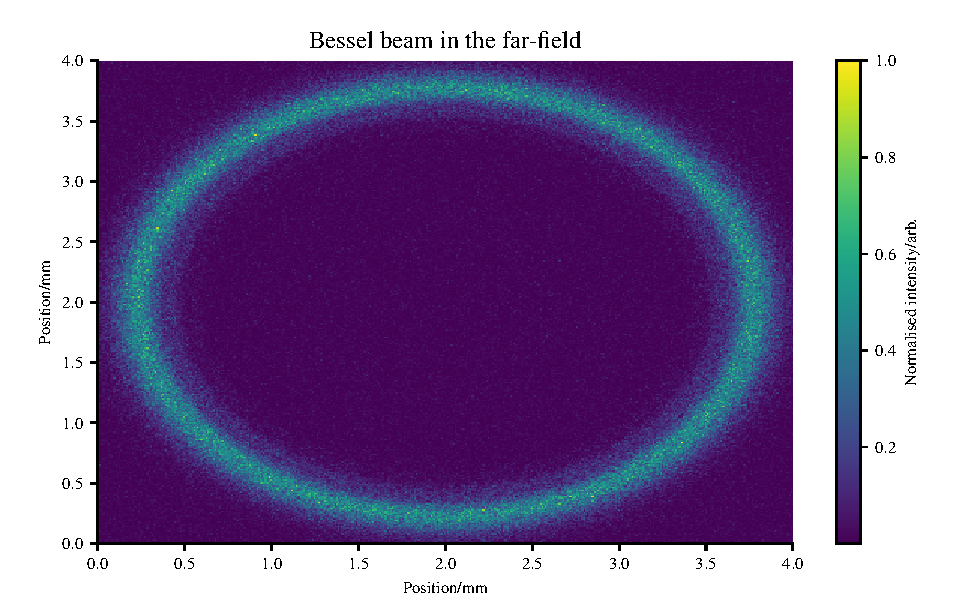
\includegraphics[scale=0.75]{far-field.pdf}
\caption{Bessel beam in the far field.}
\label{fig:farfield}
\end{figure}


a~\cite{mignon2016fractional}
\section{Conclusion}